\documentclass[diplomskirad]{fer}
% Dodaj opciju upload za generiranje konačne verzije koja se učitava na FERWeb
% Add the option upload to generate the final version which is uploaded to FERWeb

\usepackage{bm}

%--- PODACI O RADU / THESIS INFORMATION ----------------------------------------

% Naslov na hrvatskom jeziku / Title in Croatian
\naslov{Varijacijsko učenje na zašumljenim oznakama}

% Broj rada / Thesis number
\brojrada{872}

% Autor / Author
\author{Dominik Jambrović}

% Mentor 
\mentor{prof.\ dr.\ sc.\ Siniša Šegvić}

% Datum rada na hrvatskom jeziku / Date in Croatian
\datum{lipanj, 2025.}

%-------------------------------------------------------------------------------


\begin{document}


% Naslovnica se automatski generira / Titlepage is automatically generated
\maketitle


%--- ZADATAK / THESIS ASSIGNMENT -----------------------------------------------

% Zadatak se ubacuje iz vanjske datoteke / Thesis assignment is included from external file
% Upiši ime PDF datoteke preuzete s FERWeb-a / Enter the filename of the PDF downloaded from FERWeb
\zadatak{hr_0036534818_94.pdf}


%--- ZAHVALE / ACKNOWLEDGMENT --------------------------------------------------

\begin{zahvale}
  % Ovdje upišite zahvale / Write in the acknowledgment
  Zahvale!
\end{zahvale}


% Odovud započinje numeriranje stranica / Page numbering starts from here
\mainmatter


% Sadržaj se automatski generira / Table of contents is automatically generated
\tableofcontents


%--- UVOD / INTRODUCTION -------------------------------------------------------
\chapter{Uvod}
\label{pog:uvod}
  
Duboki modeli koriste se u brojnim aspektima naše svakodnevice.\ Pri razvoju i učenju modela, pažnju prije svega posvećujemo performansama na neviđenim podatcima - želimo naučiti modele koji dobro generaliziraju.\ 
Drugim riječima, želimo da modeli daju ispravna predviđanja za viđene, ali i za neviđene podatke.\ Ovime osiguravamo da naša rješenja imaju primjenu i van laboratorijskih uvjeta u kojima se uče.\
  
U procesu razvoja modela za određeni zadatak strojnog učenja, osim odabira arhitekture, algoritma učenja i hiperparametara, veliku ulogu igraju podatci na kojima učimo.\ 
Općenito govoreći, prikupljanje i označavanje podataka jedan je od najskupljih dijelova procesa razvoja rješenja za nekih problem.\ 
Važno je da prikupljeni podatci što realističnije predstavljaju stvarne situacije s kojima će se naš model susretati tj.\ da distribucija podataka odgovara stvarnoj distribuciji situacija koje prikazuju.\ 
Dodatno, pokazuje se da duboki modeli uz dovoljan kapacitet mogu naučiti ispravno predviđati oznake čak i za nasumično označene podatke~\cite{zhang2016understanding}, tako da je veoma važno da su prikupljeni podatci što točnije označeni.\
  
Područje računalnog vida~\cite{voulodimos2018deep} bavi se razvojem algoritama i modela za brojne zadatke raspoznavanja i razumijevanja slika.\ Najčešći zadatak je klasifikacija slika - model na ulazu dobiva sliku, a na izlazu treba predvidjeti razred koji odgovara ulaznom primjeru.\ 
Iako postoje brojni skupovi slikovnih podataka koji se mogu koristiti za učenje i evaluaciju modela, za konkretne zadatke u većini slučajeva trebamo prikupiti i označiti vlastite slike.\ 
Pritom postoji nekoliko čestih opasnosti: prisutnost zatrovanih podataka~\cite{biggio2012poisoning} ili zašumljenih oznaka~\cite{gupta2019dealing}.\ 

\pagebreak

Kada govorimo o trovanju podataka, maliciozni agent u skup podataka dodaje zatrovane podatke s ciljem manipulacije izlaza naučenog modela za određene ulaze.\ 
S druge strane, anotator podataka bez zlih namjera određenim podatcima može pridijeliti netočne oznake, time dodajući podatke sa zašumljenim oznakama u skup.\ 
Kroz vrijeme, razvili su se brojni algoritmi za obranu modela od zatrovanih podataka~\cite{li2021anti, huang2022backdoor, gao2023backdoor}, kao i za učenje na zašumljenim oznakama~\cite{liu2022robust, chen2024imprecise}.\ Ipak, većina radova se fokusira na samo jedan od ovih problema, a ne na razvoj algoritma koji se može nositi s oba problema.\ 
  
Cilj ovog rada je reproducirati i poboljšati rezultate okvira za obranu od zatrovanih podataka imena VIBE (engl.\ \textit{Variational inference for backdoor elimination})~\cite{sabolic2025seal}.\ 
Osim ovoga, cilj je i primijeniti VIBE na problem zašumljenih oznaka.\ Pritom VIBE evaluiramo na nekoliko čestih vrsta trovanja odnosno zašumljivanja oznaka kako bi se osigurala robusnost okvira.\ 
Dodatno, cilj je usporediti VIBE sa stanjem tehnike (engl.\ \textit{state of the art - SotA}) za problem zašumljenih oznaka.\
%-------------------------------------------------------------------------------
\chapter{Problem zatrovanih podataka}
\label{pog:zatrovani}

Cilj dodavanja zatrovanih podataka~\cite{biggio2012poisoning} u skup je ugrađivanje stražnjih vrata (engl.\ \textit{backdoor}) u naučeni model.\ Ako napad uspije, napadač može kontrolirati izlaz modela koristeći suptilne izmjene ulaznog primjera.\ 
Općenito govoreći, stvaranje zatrovanih podataka podrazumijeva dodavanje vizualnog okidača na ulazni primjer, kao i prikladnu izmjenu oznaka.\ Pritom napadač radi izmjenu određenog udjela podataka, dok preostali podatci ostaju neizmjenjeni.\ 
Hiperparametar koji opisuje udio zatrovanih podataka zvat ćemo stopom trovanja (engl. \textit{poisoning rate}).\ Pojedine metode trovanja podataka razlikuju se po načinu dodavanja okidača tj.\ načinu izmjene ulaznih primjera, kao i po načinu izmjene oznaka.\ 
  
Kada govorimo o načinu izmjene ulaznih primjera, možemo napraviti podjelu na lokalne i globalne izmjene primjera.\ Kod lokalnih izmjena, mijenja se samo određeno područje slike, najčešće dodavanjem zadanog okidača na to područje~\cite{gu2019badnets}.\ 
S druge strane, kod globalnih izmjena se mijenja cijela slika koristeći različite tehnike poput miješanja slike s okidačem~\cite{chen2020backdoor} ili transformiranja slike na temelju zadanog deformacijskog polja~\cite{nguyen2021wanet}.\ 
Osim korištenja jednog okidača za sve zatrovane podatke, određeni napadi koriste okidače specifične za pojedini uzorak~\cite{li2021invisible}.\
  
Većinu napada možemo svrstati u jedan od dva načina izmjena oznaka: \textit{all-to-one} i \textit{all-to-all} izmjena oznaka~\cite{doan2022marksman}.\ 
Kod \textit{all-to-one} metode, primjeri dobivaju zatrovanu oznaku jednog proizvoljno odabranog razreda neovisno o originalnim oznakama pojedinih primjera.\ 
S druge strane, kod \textit{all-to-all} metode, primjeri dobivaju zasebne zatrovane oznake ovisno o originalnim oznakama.\ 
Osim ova dva načina izmjena oznaka, određeni napadi uopće ne mijenjaju oznake zatrovanih primjera, već se oslanjaju isključivo na jače izmjene ulaznih primjera.\ Ovakve napade zovemo napadi s čistim oznakama (engl. \textit{clean-label attacks})~\cite{barni2019new}.\
  
Uspješnost pojedinog napada mjerimo metrikom imena stopa uspješnosti napada (engl.\ \textit{attack success rate} - ASR).\ Ovu mjeru definiramo kao točnost modela mjerenu isključivo na zatrovanim primjerima.\ 
Cilj algoritama za obranu od zatrovanih podataka je naučiti čisti model na zatrovanom skupu.\ Drugim riječima, glavni cilj obrane je naučiti model koji ima izvrsne performanse na čistim podatcima, ali i što nižu stopu uspješnosti napada.\ 

\section{Primjeri metoda trovanja podataka}
\label{sek:primjeri_trovanja}

U ovome radu, fokusiramo se na tri metode trovanja podataka: napade BadNets~\cite{gu2019badnets}, Blend~\cite{chen2020backdoor} te WaNet~\cite{nguyen2021wanet}.\
  
\subsection{Napad BadNets}
\label{sub:badnets}

Napad BadNets uobičajeno dodaje jedan zadani okidač na svaki odabrani ulazni primjer.\ Okidač možemo shvatiti kao uzorak piksela koji se dodaje na specifično mjesto na slici.\ 
Na primjer, okidač može biti bijeli pravokutnik pozicioniran u donjem lijevom kutu slike.\ Naravno, korišteni uzorak može biti proizvoljne kompleksnosti i veličine.\ 
Kod napada BadNets, izmjene oznaka su najčešće tipa \textit{all-to-one}, ali česte su i izmjene tipa \textit{all-to-all}.\

\begin{figure}[h]
  \centering
  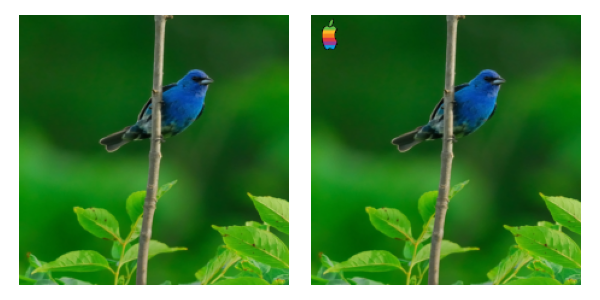
\includegraphics[scale=0.6]{./Slike/imagenet1k_uzorak_badnets.png}
  \caption{Primjer primjene napada BadNets.\ Izvornoj slici (lijevo) dodaje se okidač kako bi nastala zatrovana slika (desno).}
  \label{fig:badnets}
\end{figure}

\pagebreak
  
\subsection{Napad Blend}
\label{sub:blend}

Napad Blend provodi miješanje zadanog okidača sa svakim odabranim ulaznim primjerom.\ Pritom je jačina napada određena hiperparametrom $\alpha$ koji nazivamo jačina miješanja (engl.\ \textit{blending strength}).\ 
Primjenu napada Blend možemo prikazati jednadžbom:

\begin{equation}
  \bm{\tilde{x}} = (1 - \alpha) \cdot \bm{x} + \alpha \cdot \bm{t}
  \label{eq:blend}
\end{equation}

Pri čemu $\bm{x}$ označava ulazni primjer, $\bm{t}$ okidač, a $\bm{\tilde{x}}$ zatrovani primjer.\ Kod napada Blend, izmjene oznaka su uobičajeno tipa \textit{all-to-one}.\

\begin{figure}[h]
  \centering
  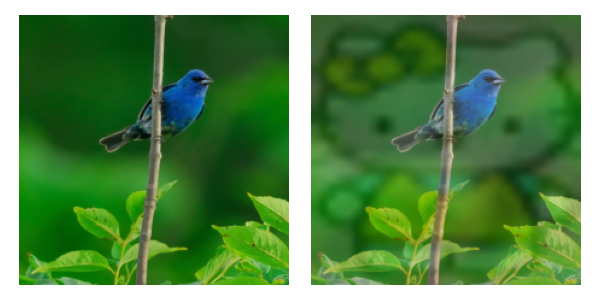
\includegraphics[scale=0.6]{./Slike/imagenet1k_uzorak_blend.png}
  \caption{Primjer primjene napada Blend.\ Izvorna slika (lijevo) miješa se s okidačem uz $\alpha = 0.2$ kako bi nastala zatrovana slika (desno).}
  \label{fig:blend}
\end{figure}
  
\subsection{Napad WaNet}
\label{sub:wanet}

Napad WaNet provodi geometrijsku transformaciju svakog odabranog ulaznog primjera koristeći nasumično generirano deformacijsko polje.\ Deformacijsko polje svakom pikselu odredišne slike dodjeljuje vektor pomaka prema pikselu izvorne slike.\
Pritom hiperparametar $k$ određuje veličinu nasumično generiranog polja šuma na temelju kojeg se skaliranjem i interpolacijom dobiva konačno deformacijsko polje, a hiperparametar $s$ određuje jačinu deformacije.\ 
Primjenu napada WaNet možemo definirati jednadžbom:

\begin{equation}
  \bm{\tilde{x}} = \mathcal{W}(\bm{x}, \bm{M}(k, s))
  \label{eq:wanet}
\end{equation}

\pagebreak

Pri čemu $\bm{x}$ označava ulazni primjer, $\bm{M}$ deformacijsko polje generirano uz hiperparametre $k$ i $s$, $\mathcal{W}$ primjenu deformacijskog polja na ulazni primjer, a $\bm{\tilde{x}}$ zatrovani primjer.\ 
Kao i kod napada Blend, kod napada WaNet su izmjene oznaka uobičajeno tipa \textit{all-to-one}.\ 

\begin{figure}[h]
  \centering
  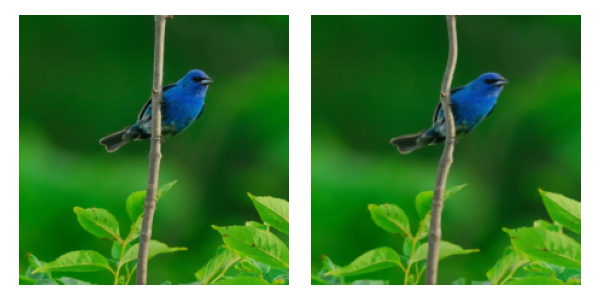
\includegraphics[scale=0.6]{./Slike/imagenet1k_uzorak_wanet.png}
  \caption{Primjer primjene napada WaNet.\ Izvorna slika (lijevo) transformira se koristeći deformacijsko polje uz $k = 8$ i $s = 4$ kako bi nastala zatrovana slika (desno).\ Hiperparametri $k$ i $s$ su uvećani kako bi učinak trovanja bio uočljiviji.}
  \label{fig:wanet}
\end{figure}

\section{Primjeri algoritama za obranu od zatrovanih podataka}
\label{sek:primjeri_obrana_trovanje}

U ovome radu, rezultate okvira VIBE uspoređujemo s rezultatima triju algoritama za obranu od zatrovanih podataka: \textit{Anti-backdoor learning} (ABL)~\cite{li2021anti}, \textit{Decoupling based defense} (DBD)~\cite{huang2022backdoor} te \textit{Adaptively splitting dataset-based defense} (ASD)~\cite{gao2023backdoor}.\

\subsection{Obrana ABL}
\label{sub:abl}

Algoritam \textit{Anti-backdoor learning} (ABL) sastoji se od dva glavna koraka: izoliranje zatrovanih podataka (engl.\ \textit{backdoor isolation}) i odučavanje trovanja (engl. \textit{backdoor unlearning}).\ 
Osnovna ideja ove obrane je da se nakon određenog broja epoha učenja uz posebno definiran gubitak izolira određeni broj primjera za koje se smatra da su zatrovani.\  
Nakon prvog koraka, ti se primjeri koriste za odučavanje trovanja, dok se preostali primjeri koriste za standardno učenje.\ 
  
Konkretno, cilj prvog koraka je zadržati vrijednost gubitka svakog pojedinog primjera oko praga $\gamma$.\
Kako bi ovo postigli, autori predlažu korištenje gradijentnog uspona u slučaju da gubitak primjera padne ispod praga, dok se inače koristi gradijentni spust.\ Gubitak u prvom koraku možemo prikazati jednadžbom:

\begin{equation}
  \mathcal{L}_1 = \mathbb{E}_{(\bm{x}, \bm{y}) \sim \mathcal{D}} \left[ \operatorname{sign} \left( \ell(f_{\bm{\theta}}(\bm{x}), \bm{y}) - \gamma \right) \cdot \ell(f_{\bm{\theta}}(\bm{x}), \bm{y}) \right]
  \label{eq:abl1}
\end{equation}

Pritom $(\bm{x}, \bm{y}) \sim \mathcal{D}$ označava primjer $\bm{x}$ s pripadnom oznakom $\bm{y}$ iz skupa podataka $\mathcal{D}$, $f_{\bm{\theta}}(\bm{x})$ izlaz modela s parametrima $\bm{\theta}$, $\ell(\bm{\hat{y}}, \bm{y})$ gubitak za predviđenu oznaku $\bm{\hat{y}}$ i stvarnu oznaku $\bm{y}$, a $\operatorname{sign}$ operaciju signum.\ 
  
Ideja je da će gubitak za zatrovane primjere veoma brzo pasti ispod praga te će se za njih često aktivirati gradijentni uspon, dok će gubitak čistih primjera sporije padati i stabilizirati se oko praga.\ 
Nakon zadanog broja epoha, izolira se udio $p$ primjera s najnižim gubitkom i proglašava potencijalnim zatrovanim skupom.\ Važno je napomenuti da bismo prvi korak ABL-a mogli zamijeniti proizvoljnim algoritmom detekcije zatrovanih primjera.\ 
  
U drugom koraku, učenje se u svakoj epohi provodi zasebno za procijenjeni čisti odnosno zatrovani skup.\ 
Dok se učenje na čistom skupu provodi uz standardni gradijentni spust, učenje na zatrovanom skupu provodi se uz gradijentni uspon kako bi model odučili od trovanja.\ 
Ovo je moguće zato što je trovanje najčešće realizirano uz samo jedan ciljni razred tj.\ uz \textit{all-to-one} način izmjene oznaka.\ Gubitak u drugom koraku možemo prikazati jednadžbom:

\begin{equation}
  \mathcal{L}_2 = \mathbb{E}_{(\bm{x}, \bm{y}) \sim \hat{\mathcal{D}}_c} \left[ \ell(f_{\bm{\theta}}(\bm{x}), \bm{y}) \right] - \mathbb{E}_{(\bm{x}, \bm{y}) \sim \hat{\mathcal{D}}_b} \left[ \ell(f_{\bm{\theta}}(\bm{x}), \bm{y}) \right]
  \label{eq:abl2}
\end{equation}

Pritom $\hat{\mathcal{D}}_c$ označava procijenjeni čisti skup, a $\hat{\mathcal{D}}_b$ procijenjeni zatrovani skup.\

\subsection{Obrana DBD}
\label{sub:dbd}

Algoritam \textit{Decoupling based defense} (DBD) problem učenja modela na zatrovanim podatcima razdvaja na tri koraka.\ 
Pritom DBD model tretira kao dvije povezane cjeline: ekstraktor značajki (engl.\ \textit{feature extractor}) te klasifikator (najčešće nekoliko potpuno-povezanih slojeva).\  
Ekstraktor značajki za ulazni primjer na izlazu daje vektor značajki tj.\ ugrađivanje (engl.\ \textit{embedding}) u latentnom metričkom prostoru.\ 
S druge strane, klasifikator za ugrađivanje na ulazu predviđa jednu od mogućih oznaka.\

\begin{figure}[h]
  \centering
  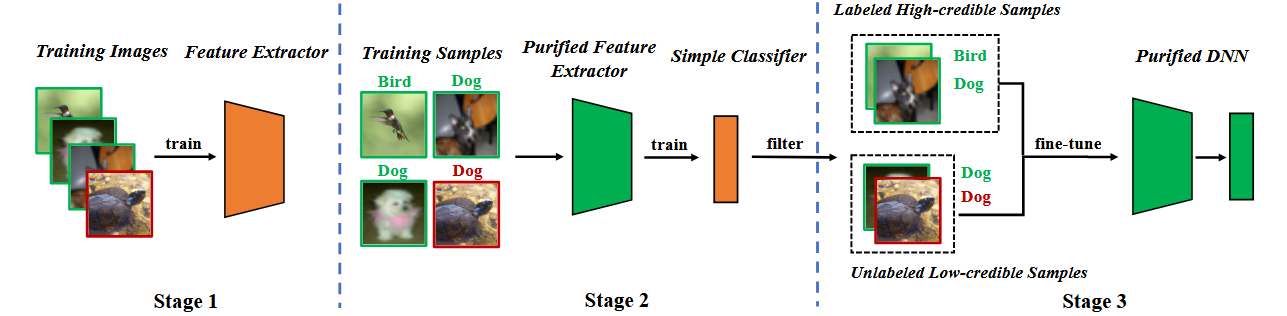
\includegraphics[scale=0.65]{./Slike/dbd.png}
  \caption{Prikaz glavnih koraka obrane DBD.\ Preuzeto iz \cite{huang2022backdoor}.}
  \label{fig:dbd}
\end{figure}
  
U prvom koraku, DBD uči ekstraktor značajki koristeći proizvoljan algoritam samonadziranog učenja~\cite{jaiswal2020survey} na slikama bez oznaka.\ 
Budući da algoritmi samonadziranog učenja uobičajeno uključuju korištenje jakih augmentacija ulaznih primjera, kvaliteta okidača kod zatrovanih primjera bit će narušena.\ 
Dodatno, jer se model u ovoj fazi uči bez oznaka, u prvom koraku nije moguće zatrovati ekstraktor značajki.\ Drugim riječima, na kraju prvog koraka imat ćemo naučen čisti ekstraktor značajki.\ 

U drugom koraku, parametri ekstraktora značajki su zamrznuti, a klasifikator učimo koristeći klasično nadzirano učenje na podatcima s oznakama.\ 
Pritom kao funkciju gubitka koristimo simetričnu unakrsnu entropiju - pokazano je da korištenje iste rezultira višim gubitkom kod zatrovanih primjera~\cite{wang2019symmetric}.\ 
Ipak, ako bismo koristili samo ova dva koraka, dobiveni model ne bi imao performanse jednake stanju tehnike jer smo ekstraktor značajki učili bez oznaka.\ 
Zbog toga, važno je napraviti podjelu skupa podataka na čisti i zatrovani skup te nakon toga ugoditi (engl.\ \textit{fine-tune}) cijeli model.\ 
Kod algoritma DBD, ova podjela se radi na temelju iznosa gubitka: udio $\alpha$ primjera s najnižim iznosom gubitka smatrat ćemo vjerodostojnim tj.\ čistim skupom, dok ćemo preostale primjere smatrati zatrovanima.\ 

Treći korak koristi podjelu na čisti i zatrovani skup kako bi dodatno ugodio parametre cijelog modela.\ 
Konkretno, zatrovanom skupu uklanjamo oznake te potom model učimo koristeći proizvoljni algoritam polunadziranog učenja~\cite{van2020survey}.\ 
Na kraju ovog koraka, imat ćemo naučen cjelokupni model otporan na zatrovane primjere.\ 

\pagebreak

\subsection{Obrana ASD}
\label{sub:asd}

Algoritam \textit{Adaptively splitting dataset-based defense} (ASD) problem učenja modela na zatrovanim podatcima razdvaja na tri koraka.\ 
Tijekom sva tri koraka, održavaju se dva skupa podataka: čisti i zagađeni skup.\ Pritom se u čistom skupu nalaze podatci za koje je velika vjerojatnost da su čisti, dok se u zagađenom skupu nalaze zatrovani podatci, kao i preostali čisti podatci.\ 
Kroz učenje, čisti skup se povećava dodavanjem primjera iz zagađenog skupa.\ Konačno, na kraju učenja bi zagađeni skup trebao sadržavati isključivo zatrovane podatke.\ 
Parametri modela uvijek se ažuriraju na temelju proizvoljnog polunadziranog gubitka, pri čemu se zagađeni skup koristi za učenje bez oznaka.\   

\begin{figure}[h]
  \centering
  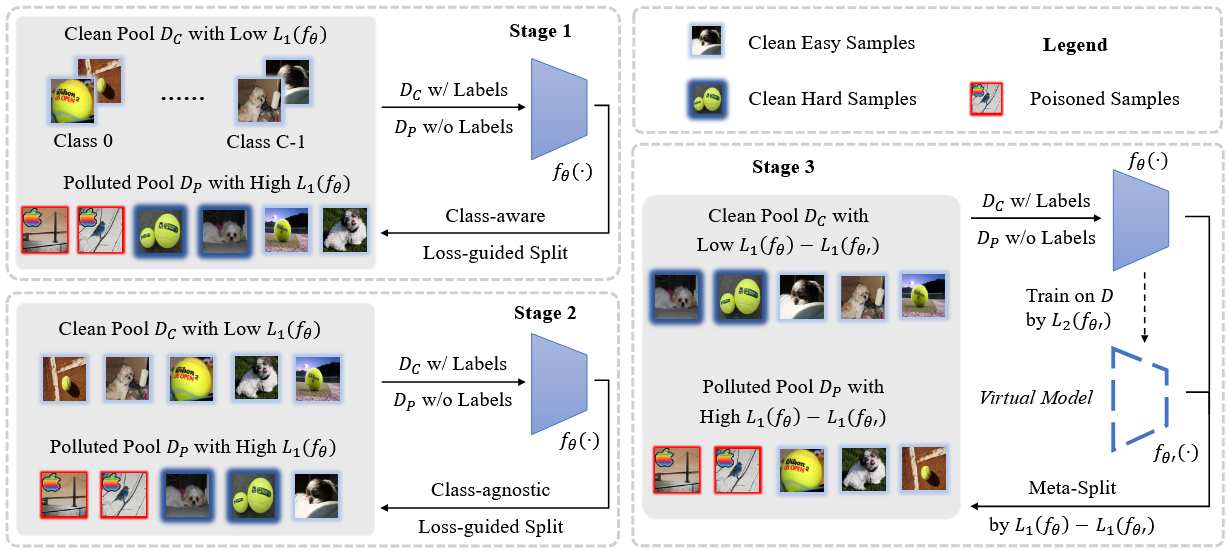
\includegraphics[scale=0.65]{./Slike/asd.png}
  \caption{Prikaz glavnih koraka obrane ASD.\ $D_C$ predstavlja čisti skup, a $D_P$ zagađeni skup.\ $\mathcal{L}_1$ odgovara gubitku $\mathcal{L}_{SCE}$, a $\mathcal{L}_2$ gubitku $\mathcal{L}_{CE}$.\ Preuzeto iz \cite{gao2023backdoor}.}
  \label{fig:asd}
\end{figure}
  
U prvom koraku, čisti skup se inicijalizira na mali broj provjereno čistih primjera (na primjer, po $10$ primjera za svaki razred), dok se zagađeni skup inicijalizira na cijeli skup podataka.\ 
Svakih $t$ epoha učenja, u čisti skup se iz zagađenog skupa dodaje $n$ primjera iz svakog pojedinog razreda koji imaju najniži gubitak $\mathcal{L}_{SCE}$.\ Pritom kao funkciju gubitka $\mathcal{L}_{SCE}$ koristimo simetričnu unakrsnu entropiju kako bi zatrovani primjeri imali što viši gubitak.\ 
Ovu podjelu zovemo razredno-svjesna podjela vođena gubitkom (engl.\ \textit{class-aware loss-guided split}).\ 
  
Tijekom drugog koraka, čisti skup značajno proširujemo dodavanjem udjela $\alpha$ zagađenog skupa.\ 
Pritom se dodaju primjeri iz cijelog skupa (neovisno o razredu) koji imaju najniži gubitak $\mathcal{L}_{SCE}$.\ 
Ovu podjelu zovemo razredno-nesvjesna podjela vođena gubitkom (engl.\ \textit{class-agnostic loss-guided split}).\ 
  
Nakon prva dva koraka ASD-a, u zagađenom skupu preostaju zatrovani primjeri, ali i neki teški primjeri specifični za model.\ 
Zbog toga što model nismo učili na teškim primjerima s oznakama, performanse modela trenutno su niže od stanja tehnike.\ Kako bismo dodali i teške primjere u čisti skup, svaku epohu trećeg koraka konstruiramo virtualni model.\ 
Virtualni model inicijaliziramo parametrima glavnog modela te potom provodimo jednu epohu nadziranog učenja na zagađenom skupu uz korištenje gubitka $\mathcal{L}_{CE}$.\ Kao funkciju gubitka $\mathcal{L}_{CE}$ koristimo standardnu unakrsnu entropiju.\ 
Nakon učenja virtualnog modela, mjerimo smanjenje gubitka definirano jednadžbom:

\begin{equation}
  \Delta \mathcal{L}_{SCE} = \mathcal{L}_{SCE}(f_{\bm{\theta}}) - \mathcal{L}_{SCE}(f_{\bm{\theta'}})
  \label{eq:asd}
\end{equation}

Pritom $f_{\bm{\theta}}$ označava glavni model s parametrima $\bm{\theta}$, a $f_{\bm{\theta'}}$ predstavlja virtualni model s parametrima $\bm{\theta'}$ dobivenim nakon jedne epohe nadziranog učenja na zagađenom skupu.\ 
Konačno, udio $\gamma$ primjera s najmanjim smanjenjem gubitka dodajemo u čisti skup.\ Intuicija iza ove podjele je da su zatrovani podatci lagani za naučiti, tako da već nakon jedne epohe nadziranog učenja isti imaju veoma nizak gubitak, dok teški čisti primjeri i dalje imaju visok gubitak.\ 
Važno je napomenuti da se virtualni model koristi isključivo za provođenje podjele na temelju smanjenja gubitka.\ 
Ovu podjelu zovemo meta-podjela (engl.\ \textit{meta-split}) jer je pristup s učenjem virtualnog modela inspiriran područjem meta-učenja (engl.\ \textit{meta-learning})~\cite{vilalta2002perspective}.\
Na kraju trećeg koraka, u čistom skupu će se nalaziti gotovo svi čisti primjeri, a dobiveni model će imati izvrsne performanse uz otpornost na zatrovane primjere.\

%-------------------------------------------------------------------------------
\chapter{Problem zašumljenih oznaka}
\label{pog:zasumljeni}

Proces stvaranja skupa vizualnih podataka otprilike možemo podijeliti u tri koraka.\ U prvom koraku, potrebno je definirati skup razreda tj.\ oznaka koje mogu biti dodijeljene svakom primjeru.\ 
Tijekom drugog koraka, cilj nam je prikupiti što veći skup slika, pritom pazeći na to da slike precizno prikazuju situacije s kojima će se naš model susretati.\ Dodatno, veoma je važno da je prikupljeni skup što raznovrsniji kako bi model mogao naučiti dobro generalizirati.\ 
Konačno, u trećem koraku anotatori označavaju slike na temelju definiranog skupa oznaka.\ Drugi i treći korak ovog procesa mogu se provoditi jedan za drugim, ali i paralelno - nakon što se prikupi određen broj slika, taj skup se šalje na označavanje, a istovremeno je moguće prikupiti još slika.\ 
  
Iako anotatori podataka prolaze kroz brojne edukacije kako bi se što bolje upoznali s pravilima na temelju kojih će označavati podatke, određeni podatci su prirodom teži od drugih pa može doći do pogrešnog označavanja.\ 
Problem zašumljenih oznaka sličan je problemu zatrovanih podataka po tome što se kod oba problema model mora nositi s pogrešnim oznakama.\ Ipak, kod problema zašumljenih oznaka podrazumijevamo da su ulazne slike netaknute tj.\ da ne postoji nikakva izmjena ulaza.\ 
Dodatno, kod problema zašumljenih oznaka ne postoji konkretan cilj - podatci sa zašumljenim oznakama nastaju slučajno, bez ikakvih loših namjera.\ 
  
Dok je kod zatrovanih podataka problem prelako učenje poveznice između prisutnosti okidača i određenog ciljnog razreda, kod podataka sa zašumljenim oznakama je problem činjenica da model uz dovoljan kapacitet može naučiti oznake čak i ako su one nasumično generirane~\cite{zhang2016understanding}.\ 
Drugim riječima, ako nismo oprezni, lako je doći do prenaučenosti (engl.\ \textit{overfitting}) modela.\ Naravno, ovakav model će loše generalizirati na ispravno označenim podatcima.\ 
  
Kako bismo mogli usporediti performanse različitih algoritama za učenje na zašumljenim oznakama, najčešće određenom udjelu čistog skupa podataka dodajemo sintetičke zašumljene oznake.\ 
Hiperparametar koji opisuje udio podataka sa zašumljenim oznakama zvat ćemo stopa šuma (engl. \textit{noise rate}).\ Nakon učenja na zašumljenim podatcima, performanse modela evaluiramo na čistom, ali i na u potpunosti zašumljenom skupu.\ 
Cilj algoritama za učenje na zašumljenim oznakama tada je zadržati performanse modela učenog na zašumljenim podatcima što bližima performansama modela učenog na čistim podatcima.\ 

\section{Primjeri metoda zašumljivanja oznaka}
\label{sek:primjeri_zasumljivanja}

U ovome radu, fokusiramo se na dvije metode zašumljivanja oznaka: simetrično (engl.\ \textit{symmetric}) i asimetrično (engl.\ \textit{asymmetric}) zašumljivanje~\cite{cordeiro2020survey}.\

\subsection{Simetrično zašumljivanje}
\label{sub:sym}

Kod simetričnog zašumljivanja, nasumično biramo zadani udio primjera iz čistog skupa podataka te istima dodjeljujemo nasumično generirane nove oznake.\ 
Ovu metodu zašumljivanja također zovemo i uniformno zašumljivanje jer svaki razred ima jednaku vjerojatnost postati nova oznaka za neki zadani primjer.\ 
  
Pritom razlikujemo dvije vrste simetričnog zašumljivanja: inkluzivnu (engl.\ \textit{symm-inc}) i ekskluzivnu (engl.\ \textit{symm-exc}) vrstu~\cite{cordeiro2020survey}.\ 
Ako govorimo o inkluzivnom simetričnom zašumljivanju, stvarna oznaka za neki zadani primjer može biti odabrana i kao zašumljena oznaka.\ 
S druge strane, kod ekskluzivnog simetričnog zašumljivanja ignoriramo stvarnu oznaku tj.\ zašumljena oznaka se uvijek razlikuje od stvarne oznake primjera.\ 
U našem radu, fokusiramo se na inkluzivno simetrično zašumljivanje.\ 

\pagebreak

\begin{figure}[h]
  \centering
  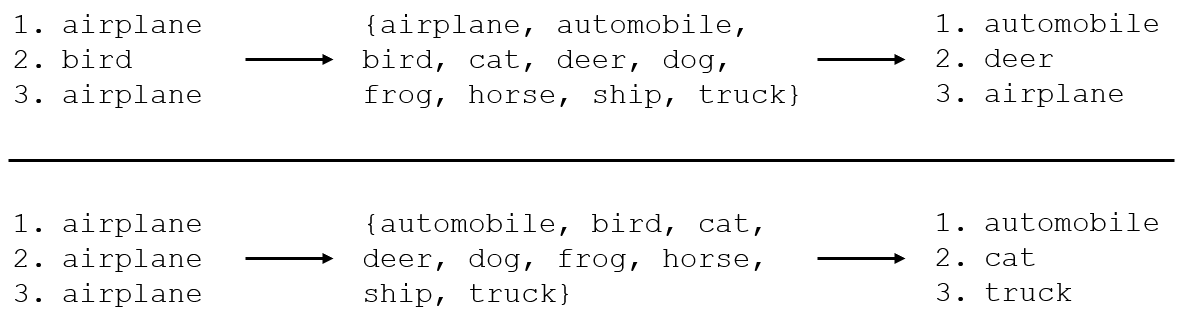
\includegraphics[scale=0.7]{./Slike/sym.png}
  \caption{Prikaz inkluzivnog (gore) odnosno ekskluzivnog (dolje) simetričnog zašumljivanja za tri odabrana primjera iz skupa CIFAR10~\cite{krizhevsky2009learning}.\ Čiste oznake (lijevo) preslikavaju se na jednu od mogućih oznaka (sredina) i nastaju zašumljene oznake (desno).\ Vidimo da primjeri s istim čistim oznakama nemaju nužno i iste zašumljene oznake.}
  \label{fig:sym}
\end{figure}

\subsection{Asimetrično zašumljivanje}
\label{sub:asym}

Kod asimetričnog zašumljivanja, prvo nasumično biramo zadani udio primjera zasebno za svaki razred.\ 
Drugim riječima, ako je u pitanju skup CIFAR10~\cite{krizhevsky2009learning}, za svaki od $10$ razreda nasumično ćemo odabrati zadani udio primjera kojima ćemo potencijalno dodijeliti zašumljene oznake.\ 

Nakon početnog odabira, svakom primjeru dodjeljujemo novu oznaku na temelju predodređenog preslikavanja.\ 
Pritom je moguće da određeni razredi nemaju definirano preslikavanje u neki drugi razred, tako da odabranim primjerima iz tih razreda neće biti dodijeljene zašumljene oznake.\ 
Preslikavanje na temelju kojeg se pojedinim primjerima dodjeljuje nova oznaka unaprijed je definirano za pojedine skupove podataka poput skupova MNIST~\cite{deng2012mnist}, CIFAR10 i CIFAR100~\cite{krizhevsky2009learning}.\ 
Kod skupova s hijerarhijskim odnosom razreda poput skupa CIFAR100, preslikavanja su definirana nasumično unutar pojedinih grupa razreda.\ 

\begin{figure}[h]
  \centering
  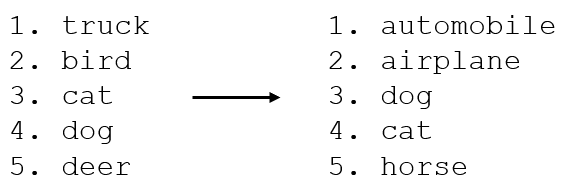
\includegraphics[scale=0.7]{./Slike/asym.png}
  \caption{Prikaz preslikavanja razreda za skup CIFAR10.\ Odabranim primjerima se na temelju čistih oznaka (lijevo) dodjeljuju zašumljene oznake (desno).\ Pritom odabrani primjeri s istim čistim oznakama uvijek imaju i iste zašumljene oznake.}
  \label{fig:asym}
\end{figure}

\pagebreak

\section{Primjeri algoritama za učenje na zašumljenim oznakama}
\label{sek:primjeri_obrana_zasumljivanje}

U ovome radu, rezultate prilagođenog okvira VIBE uspoređujemo s rezultatima dvaju algoritama za učenje na podatcima sa zašumljenim oznakama: \textit{Sparse over-parameterization} (SOP)~\cite{liu2022robust} te \textit{Imprecise label learning} (ILL)~\cite{chen2024imprecise}.\ 

\subsection{Algoritam SOP}
\label{sub:sop}

Osnovna ideja algoritma \textit{Sparse over-parameterization} (SOP) bazira se na činjenici da su primjeri sa zašumljenim oznakama u većini slučajeva rijetki.\ 
Jedan od mogućih načina za učenje modela na zašumljenim oznakama tada je modeliranje šuma za pojedine primjere koristeći rijetke vektore.\ 

Konkretno, za svaki primjer $(\bm{x}_i, \bm{y}_i)$ iz skupa podataka $\mathcal{D}$ definiramo rijetki vektor $\bm{s}_i$ koji služi kao odstupanje između uočene (potencijalno zatrovane) oznake $\bm{y}_i$ i čiste (skrivene) oznake $\bm{l}_i$.\ 
Uobičajeno, učenje modela se svodi na potragu za parametrima $\bm{\theta}$ koji minimiziraju gubitak definiran jednadžbom:

\begin{equation}
  \mathcal{L} = \mathbb{E}_{(\bm{x}, \bm{y}) \sim \mathcal{D}} \left[ \ell(f_{\bm{\theta}}(\bm{x}), \bm{y}) \right]
  \label{eq:sop1}
\end{equation}

Pritom $f_{\bm{\theta}}$ predstavlja model s parametrima $\bm{\theta}$, a $\ell(\bm{\hat{y}}, \bm{y})$ funkciju gubitka između predviđanja modela $\bm{\hat{y}}$ i dane oznake $\bm{y}$.\ 
Uz uvođenje rijetkog vektora $\bm{s}_i$ za svaki primjer, učenje se svodi na potragu za parametrima $(\bm{\theta}, \{\bm{s}_i\}_{i=1}^N)$ koji minimiziraju gubitak:

\begin{equation}
  \mathcal{L}_{SOP} = \mathbb{E}_{(\bm{x}, \bm{y}) \sim \mathcal{D}} \left[ \ell(f_{\bm{\theta}}(\bm{x}) + \bm{s}, \bm{y}) \right]
  \label{eq:sop2}
\end{equation}

Dodatno, kako bi se osigurala rijetkost vektora $\bm{s}_i$, isti definiramo pomoću vektora $\bm{u}_i$ i vektora $\bm{v}_i$ kao:

\begin{equation}
  \bm{s}_i = \bm{u}_i \odot \bm{u}_i - \bm{v}_i \odot \bm{v}_i
  \label{eq:sop_s1}
\end{equation}

Drugim riječima, za svaki podatak $(\bm{x}_i, \bm{y}_i)$ definiramo dva vektora parametara: $\bm{u}_i$ i $\bm{v}_i$.\ 
Ove vektore učimo zajedno s parametrima modela $\bm{\theta}$ koristeći gradijentni spust.\ 
Pritom je stopa učenja za parametre $\{\bm{u}_i,\bm{v}_i\}_{i=1}^N$ skalirana hiperparametrom $\alpha$ kako bi se izbjeglo trivijalno rješenje optimizacijskog problema kod kojeg vrijedi $\bm{u}_i \equiv \bm{v}_i \equiv \bm{0}\:,\:\forall i \in N$.\ 

Uočimo da vektor $\bm{s}_i$ za primjer $(\bm{x}_i, \bm{y}_i)$ dodatno mora poštovati nekoliko uvjeta: u vektoru $\bm{s}_i$ se pozitivna vrijednost može nalaziti isključivo na mjestu koje odgovara nenegativnoj vrijednosti u $\bm{y}_i$, dok se negativne vrijednosti mogu nalaziti isključivo na mjestima koje odgovaraju vrijednosti $0$ u $\bm{y}_i$.\ 
Dodatno, svaki element vektora $\bm{s}_i$ mora biti u rasponu $\left[ -1, 1 \right]$.\ Kako bismo ovo osigurali, uvodimo konačnu definiciju vektora $\bm{s}_i$:

\begin{equation}
  \bm{s}_i = \bm{u}_i \odot \bm{u}_i \odot \bm{y}_i - \bm{v}_i \odot \bm{v}_i \odot (\bm{1} - \bm{y}_i)
  \label{eq:sop_s2}
\end{equation}

Pritom su vektori parametara $\bm{u}_i$ i $\bm{v}_i$ definirani kao:

\begin{equation}
  \bm{u}_i \in \left[ -1, 1 \right]^K\:,\:\bm{v}_i \in \left[ -1, 1 \right]^K
  \label{eq:sop_u,i}
\end{equation}

U algoritmu SOP, za učenje parametara $(\bm{\theta}, \{\bm{u}_i\}_{i=1}^N)$ se kao funkcija gubitka koristi standardna unakrsna entropija.\ Nažalost, unakrsna entropija se ne može koristiti za ispravno učenje parametara $\{\bm{v}_i\}_{i=1}^N$.\ 
Umjesto toga, za učenje tih parametara kao funkciju gubitka koristimo srednju kvadratnu pogrešku.\ 

Kako bi poboljšali performanse osnovnog algoritma SOP, autori predlažu dodavanje dvije nove komponente gubitka: konzistencijski gubitak (engl.\ \textit{consistency loss})~\cite{berthelot2019mixmatch} te gubitak ravnoteže razreda (engl.\ \textit{class-balance loss})~\cite{tanaka2018joint}.\ 
Inačicu algoritma koja dodatno koristi ove dvije komponente gubitka zovemo SOP+, a ista općenito postiže bolje performanse od osnovne inačice algoritma.\

\pagebreak

\subsection{Algoritam ILL}
\label{sub:ill}

Algoritam \textit{Imprecise label learning} (ILL) obuhvaća i pokušava riješiti nekoliko problema vezanih uz nesavršenosti oznaka: učenje na djelomičnim oznakama (engl.\ \textit{partial label learning})~\cite{tian2023partial}, polunadzirano učenje te učenje na zašumljenim oznakama.\ 
Konkretno, ILL sve ove probleme smatra vrstama problema nepreciznih oznaka (engl.\ \textit{imprecise labels}).\ Skup podataka tada sadrži ulazne slike $X$ i neprecizne oznake $I$, dok su čiste oznake $Y$ skrivene (latentne).\ 
Pritom su neprecizne oznake apstraktne - u stvarnosti to može biti skup oznaka (u problemu učenja na djelomičnim oznakama), ali i zašumljena oznaka (u problemu učenja na zašumljenim oznakama).\ 
Cilj učenja modela tada je pronaći parametre $\bm{\theta}$ koji maksimiziraju zajedničku vjerojatnost definiranu kao: 

\begin{equation}
  p(X, I | \bm{\theta}) = \sum_{Y} p(X, I, Y | \bm{\theta})
  \label{eq:ill_joint}
\end{equation}

Kako bismo maksimizirali logaritam očekivanja uz prisutnost latentne varijable, koristimo algoritam maksimizacije očekivanja (algoritam EM)~\cite{moon1996expectation}.\
Pritom u E koraku algoritma maksimizacije očekivanja računamo očekivanje zajedničke vjerojatnosti $p(X, I, Y | \bm{\theta})$ uz zadanu uvjetnu vjerojatnost $p(Y | X, I, \bm{\theta}^t)$ u vremenskom koraku $t$.\ 
S druge strane, u M koraku tražimo parametre $\bm{\theta}$ koji maksimiziraju donju varijacijsku granicu (engl.\ \textit{evidence lower bound} - ELBO) vjerojatnosti $p(X, I | \bm{\theta})$.\ 
Budući da se različite vrste problema razlikuju primarno po prirodi nepreciznosti oznaka, algoritmi za pojedine probleme najviše će se razlikovati u načinu izračuna vjerojatnosti $p(Y | X, I, \bm{\theta}^t)$.\
Ovime algoritam ILL pruža unificirani okvir koji podržava različite vrste nepreciznosti oznaka, kao i kombinacije istih.\

Dakle, glavni cilj algoritma ILL je pronaći parametre $\bm{\theta}$ koji maksimiziraju zajedničku vjerojatnost $p(X, I | \bm{\theta})$ odnosno logaritam iste.\
Prema algoritmu EM, ovaj problem možemo riješiti maksimizacijom očekivanja:

\begin{equation}
  \mathbb{E}_{Y | X, I, \bm{\theta}^t} \left[ \log p(X, Y, I | \bm{\theta}) \right] = \mathbb{E}_{Y | X, I, \bm{\theta}^t} \left[ \log p(Y | X, \bm{\theta}) + \log p(I | X, Y, \bm{\theta}) \right]
  \label{eq:ill_expectation}
\end{equation}

\pagebreak

Pritom ignoriramo član $p(X)$ jer isti ne ovisi o parametrima $\bm{\theta}$.\ Iz dobivenog izraza vidimo da izračunom očekivanja razmatramo sve moguće oznake $Y$ na temelju danih nepreciznih oznaka $I$, umjesto da se fokusiramo na samo jednu prepravljenu oznaku.\
Na temelju ove formulacije dalje možemo izvesti cilj za pojedini problem.\ U našem radu, fokusirat ćemo se na izvod za problem učenja na zašumljenim oznakama.\ 

Kod problema učenja na zašumljenim oznakama, neprecizne oznake $I$ se manifestiraju kao zašumljene oznake $\hat{Y}$.\ 
Vjerojatnost $p(\hat{Y} | Y, X, \bm{\theta})$ tada predstavlja model šuma ovisan o pojedinom uzorku $X$.\ 
Ovaj problem pojednostavit ćemo razmatranjem modela šuma neovisnog o uzorku $\mathcal{T}(\hat{Y} | Y, \bm{\omega})$ s parametrima $\bm{\omega}$.\ Cilj koji želimo maksimizirati tada dobivamo kao:

\begin{equation}
  \begin{aligned}
    \mathbb{E}_{Y | X, I, \bm{\theta}^t} \left[ \log p(X, Y, I | \bm{\theta}) \right] &= \mathbb{E}_{Y | X, I, \bm{\theta}^t} \left[ \log p(Y, I | X, \bm{\theta}) \right] \\
    &= \mathbb{E}_{Y | X, \hat{Y}, \bm{\theta}^t} \left[ \log p(Y, \hat{Y} | X, \bm{\theta}) \right] \\
    &= \mathbb{E}_{Y | X, \hat{Y}, \bm{\theta}^t} \left[ \log p(Y | \hat{Y}, X, \bm{\theta}) + \log p(\hat{Y} | X, \bm{\theta}) \right] \\
    &= \sum_{Y} p(Y | \hat{Y}, X, \bm{\theta}^t) \log p(Y | \hat{Y}, X, \bm{\theta}) + \log p(\hat{Y} | X, \bm{\theta}) \\
  \end{aligned}
  \label{eq:ill_target}
\end{equation}

Funkcija gubitka koju želimo minimizirati tada postaje:

\begin{equation}
  \mathcal{L}_{ILL} = \mathcal{L}_{CE} (p(\bm{y} | \bm{x}, \bm{\hat{y}}, \bm{\theta}, \bm{\omega}^t), p(\bm{y} | \bm{x}, \bm{\hat{y}}, \bm{\theta}^t, \bm{\omega}^t)) + \mathcal{L}_{CE} (p(\bm{\hat{y}} | \bm{x}, \bm{\theta}, \bm{\omega}), \bm{\hat{y}})
  \label{eq:ill_loss}
\end{equation}

Pritom $\mathcal{L}_{CE}$ označava unakrsnu entropiju.\ Prva komponenta dobivenog gubitka odgovara konzistencijskom gubitku čistih oznaka uvjetovanih zašumljenim oznakama, dok druga komponenta odgovara nadziranom gubitku na zašumljenim oznakama.\ 
Pritom se za izračun obje komponente koristi model šuma uz zadanu zašumljenu oznaku $\bm{\hat{y}}$:

\begin{equation}
  \begin{aligned}
    p(\bm{y} | \bm{x}, \bm{\hat{y}}, \bm{\theta}, \bm{\omega}^t) \propto p(\bm{y} | \bm{x}, \bm{\theta}) \, \mathcal{T}(\bm{\hat{y}} | \bm{y}, \bm{\omega}^t) \\
    p(\bm{\hat{y}} | \bm{x}, \bm{\theta}, \bm{\omega}) = \sum_{\bm{y}} p(\bm{y} | \bm{x}, \bm{\theta}) \, \mathcal{T}(\bm{\hat{y}} | \bm{y}, \bm{\omega})
  \end{aligned}
  \label{eq:ill_probs}
\end{equation}

%-------------------------------------------------------------------------------
\chapter{Samonadzirano učenje}
\label{pog:samonadzirano}

Samonadzirano učenje~\cite{jaiswal2020survey} paradigma je strojnog učenja kod koje model uči izlučivati korisne reprezentacije tj.\ značajke ulaznih podataka na temelju posebno osmišljenih zadataka bez oznaka (engl.\ \textit{pretext tasks}).\ 
Ovim pristupom pokušava se adresirati problem cijene i vremena potrebnog za označavanje velikih skupova podataka.\ 
Model učen proizvoljnim algoritmom samonadziranog učenja dalje se može koristiti kao okosnica (engl.\ \textit{backbone}) za model koji rješava neki nizvodni (engl.\ \textit{downstream}) zadatak poput klasifikacije ili detekcije objekata.\ 
Pritom se okosnici dodaje klasifikacijska glava (najčešće nekoliko potpuno-povezanih slojeva), a cijeli model se dodatno ugađa nadziranim učenjem na manjem skupu podataka prilagođenom konkretnom problemu.\ 
  
Ključno pitanje kod samonadziranog učenja je formiranje zadatka učenja bez oznaka tj.\ odlučivanje o tome na temelju čega će model dobivati signal za učenje.\ 
Tipični zadatci uključuju rekonstrukciju ulaznih podataka na temelju izlučenih reprezentacija, grupiranje reprezentacija tj.\ ugrađivanja (engl.\ \textit{embedding}) semantički sličnih podataka u prostoru ugrađivanja ili predviđanje maskiranih piksela ulaznih slika (engl.\ \textit{masked image modeling} - MIM)~\cite{hondru2024masked}.\
Rješavanjem jednog od zadataka učenja, model posredno uči izlučivati korisne reprezentacije ulaznih podataka ili uočavati korisne odnose između podataka.\ 
  
Područje samonadziranog učenja možemo podijeliti na temelju korištenog tipa zadatka učenja, a neka od najpoznatijih područja su autoasocijativno samonadzirano učenje~\cite{kramer1991nonlinear} i kontrastno samonadzirano učenje~\cite{jaiswal2020survey}.\ 
Kod autoasocijativnog samonadziranog učenja, osnovni zadatak je rekonstruirati ulazni podatak na temelju izlučene reprezentacije.\ Pritom je model koji učimo odgovoran za izlučivanje reprezentacije, dok za rekonstrukciju uobičajeno koristimo drugi model koji nakon učenja odbacujemo.\
U našem radu, fokusirat ćemo se na kontrastno samonadzirano učenje.\ 

\section{Kontrastno samonadzirano učenje}
\label{sek:contrastive}

Kontrastno učenje jedno je od područja samonadziranog učenja.\ Ono podrazumijeva učenje izlučivanja korisnih reprezentacija tj.\ ugrađivanja ulaznih podataka na temelju parova podataka.\ 
Ako su dobivena ugrađivanja normirana, a sličnost dvaju ugrađivanja možemo izračunati koristeći neku od standardnih metrika (na primjer, kosinusnu sličnost), tada govorimo o metričkim ugrađivanjima tj.\ ugrađivanjima u metrički prostor~\cite{chavez2001searching}.\ 
Možemo reći da naučeni model preslikava ulazne slike na $(d - 1)$ dimenzionalnu hipersferu $S^{d - 1}$, pri čemu sličnost ugrađivanja odgovara semantičkoj sličnosti ulaza.\
  
Kod kontrastnog učenja razlikujemo sidro, pozitivne i negativne primjere.\ Trenutno promatrani podatak iz minigrupe nazivamo sidro, podatak sličan sidru nazivamo pozitivan primjer, a podatak različit od sidra nazivamo negativan primjer.\ 
Budući da primjeri nisu označeni, pozitivne primjere najčešće dobivamo perturbacijom sidra, dok negativnim primjerima smatramo sve ostale podatke iz minigrupe.\ 

\begin{figure}[h]
  \centering
  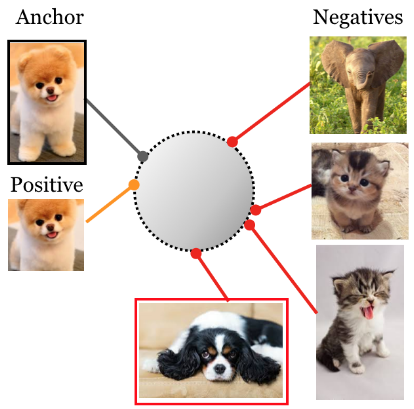
\includegraphics[scale=1]{./Slike/ssl.png}
  \caption{Prikaz osnovne ideje kontrastnog samonadziranog učenja. Cilj učenja je približiti sidro (gore lijevo) i pozitivan primjer (dolje lijevo), ali i međusobno udaljiti sidro i negativne primjere (desno).\ Preuzeto iz \cite{khosla2020supervised}.}
  \label{fig:ssl}
\end{figure}

Glavni cilj kontrastnog učenja je približiti ugrađivanja pozitivnih parova (sidra i pozitivnog primjera), ali i istovremeno udaljiti ugrađivanja negativnih parova (sidra i negativnih primjera).\ 
Kako bismo ovo postigli, veoma je važno prikladno definirati funkciju gubitka, a neke od mogućih su trojni gubitak~\cite{schroff2015facenet} te gubitak N parova.\ 
Gubitak N parova također je poznat i kao infoNCE gubitak~\cite{oord2018representation}, a možemo ga definirati jednadžbom:

\begin{equation}
  \mathcal{L}_{infoNCE} = - \log{\frac{\exp(\langle \bm{z}_{a}, \bm{z}_{p} \rangle / \tau)}{\sum_{i=1}^{N}{\exp(\langle \bm{z}_{a}, \bm{z}_{ni} \rangle / \tau)}}}
  \label{eq:infoNCE}
\end{equation}

Pritom $\bm{z}_{a}$ označava ugrađivanje sidra $\bm{x}_{a}$, $\bm{z}_{p}$ ugrađivanje pozitivnog primjera $\bm{x}_{p}$, $\bm{z}_{ni}$ ugrađivanje i-tog negativnog primjera $\bm{x}_{ni}$ iz minigrupe, a $\tau$ hiperparametar temperature.\ 
Oznaka $\langle ... \rangle$ označava skalarni produkt vektora unutar zagrada.\
  
U algoritmu za obranu od zatrovanih podataka VIBE, samonadzirana inicijalizacija parametara modela veoma je važan korak koji osigurava uspješnost obrane.\ 
Pritom za inicijalizaciju koristimo okvir All4One~\cite{estepa2023all4one} koji se bazira na kontrastnom samonadziranom učenju.\

\section{Okvir All4One}
\label{sek:all4one}

Okvir All4One kombinira tri zasebna pristupa kontrastiranju kako bi naučeni modeli postizali što bolje rezultate.\ 
Konkretno, optimizacijski cilj okvira All4One sadrži komponentu kontrastiranja najbližih susjeda (engl.\ \textit{nearest neighbour contrast})~\cite{dwibedi2021little}, komponentu kontrastiranja centroida (engl.\ \textit{centroid contrast}) te komponentu kontrastiranja značajki (engl.\ \textit{feature contrast})~\cite{zbontar2021barlow}.\ 

\begin{figure}[h]
  \centering
  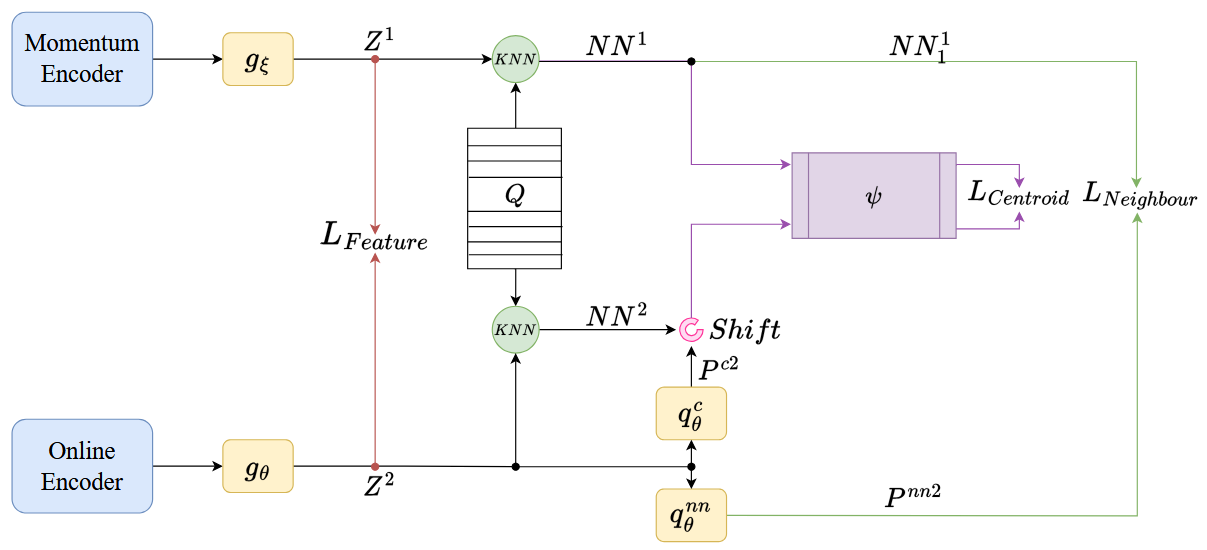
\includegraphics[scale=0.7]{./Slike/all4one.png}
  \caption{Prikaz arhitekture okvira All4One. Komponenta kontrastiranja najbližih susjeda označena je zelenom bojom, komponenta kontrastiranja centroida ljubičastom bojom, a komponenta kontrastiranja značajki crvenom bojom.\ Preuzeto iz \cite{estepa2023all4one}.}
  \label{fig:all4one}
\end{figure}

\pagebreak

U okviru All4One, model koji učimo služi kao koder značajki $f_{\bm{\theta}}$.\ Osim glavnog kodera koji učimo gradijentnim spustom, tijekom učenja se dodatno održava i koder s momentom $f_{\bm{\xi}}$ čiji parametri odgovaraju eksponencijalnom pomičnom prosjeku (engl.\ \textit{exponential moving average} - EMA) parametara glavnog kodera.\
Dodatno, osim para kodera, učimo i par projektora $g_{\bm{\theta}}$ i $g_{\bm{\xi}}$.\ Za svaku sliku $\bm{x}$ na ulazu, generiraju se dvije augmentirane slike $\bm{x}^1$ te $\bm{x}^2$.\ 
Jedna od dobivenih augmentiranih slika tada prolazi kroz koder s momentom i pripadni projektor te dobivamo ugrađivanje $\bm{z}^1 = g_{\bm{\xi}}(f_{\bm{\xi}}(\bm{x}^1))$, dok druga augmentirana slika prolazi kroz glavni koder i pripadni projektor te dobivamo ugrađivanje $\bm{z}^2 = g_{\bm{\theta}}(f_{\bm{\theta}}(\bm{x}^2))$.\
Dobivena ugrađivanja dalje se mogu koristiti za izračun pojedinih komponenti optimizacijskog cilja.\ Osim para kodera i para projektora, dodatno se održavaju i dva prediktora $q_{\bm{\theta}}^{nn}$ te $q_{\bm{\theta}}^{c}$ koji služe za prilagodbu ugrađivanja za zadatak kontrastiranja najbližih susjeda odnosno zadatak kontrastiranja centroida.\

\subsection{Kontrastiranje najbližih susjeda}
\label{sub:knn}

Kontrastiranje najbližih susjeda često je korišten pristup kontrastnog samonadziranog učenja kod kojega se ugrađivanje jedne od perturbiranih slika zamijeni sa svojim najbližim susjedom.\ 
Konkretno, tijekom učenja održavamo skup prethodnih ugrađivanja (engl.\ \textit{support set}) $Q$ koji možemo koristiti za pronalazak najbližih susjeda za neko zadano ugrađivanje.\ Ovu operaciju označit ćemo operatorom $KNN$.\ 
Gubitak za i-ti primjer $\bm{x}_i$ u minigrupi tada možemo definirati jednadžbom:

\begin{equation}
  \mathcal{L}_{NNCLR} = - \log{\frac{\exp(\langle \bm{nn}_{i}^{1}, \bm{p}_{i}^{nn, 2} \rangle / \tau)}{\sum_{k=1}^{N}{\exp(\langle \bm{nn}_{i}^{1}, \bm{p}_{k}^{nn, 2} \rangle / \tau)}}}
  \label{eq:NNCLR_loss}
\end{equation}

Pritom $\bm{nn}_{i}^{1}$ označava najbližeg susjeda ugrađivanja prve perturbacije primjera $\bm{x}_i$, $\bm{p}_{i}^{nn, 2}$ izlaz prediktora $q_{\bm{\theta}}^{nn}$ za ugrađivanje druge perturbacije primjera $\bm{x}_i$, a $\tau$ hiperparametar temperature.\ 
Naspram osnovne inačice kontrastnog učenja, kontrastiranje najbližih susjeda povećava raznolikost primjera koje model vidi tijekom učenja, a time i generalizacijsku moć naučenog modela.\ 

\pagebreak

\subsection{Kontrastiranje centroida}
\label{sub:centroids}
  
Ipak, pokazano je da modeli učeni kontrastiranjem najbližih susjeda mogu postići još bolje performanse ako se pritom koristi više od jednog najbližeg susjeda~\cite{koohpayegani2021mean}.\ 
Nažalost, učenje s više od jednog najbližeg susjeda značajno povećava trajanje učenja jer se funkcija cilja treba evaluirati za svakog susjeda pojedinačno.\ 
Autori okvira All4One ovome problemu doskaču uvođenjem kontrastiranja centroida.\ 

\begin{figure}[h]
  \centering
  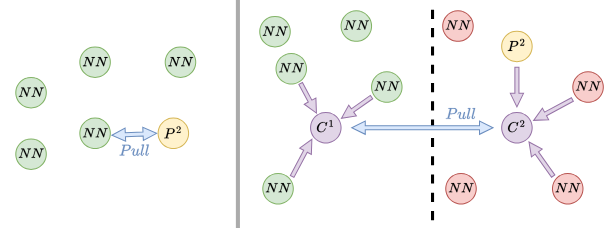
\includegraphics[scale=1]{./Slike/neighbour_vs_centroid.png}
  \caption{Prikaz kontrastiranja najbližih susjeda (lijevo) i kontrastiranja centroida (desno).\ Kod kontrastiranja najbližih susjeda, kontrastiraju se najbliži susjed jedne perturbacije i druga perturbacija.\ S druge strane, kod kontrastiranja centroida, kontrastiraju se centroidi pojedinih perturbacija.\ Preuzeto iz \cite{estepa2023all4one}.}
  \label{fig:neighbour_vs_centroid}
\end{figure}

Konkretno, nakon što smo za zadani primjer $\bm{x}$ generirali ugrađivanja $\bm{z}^1$ te $\bm{z}^2$, za ista prvo pronalazimo skupove najbližih susjeda $NN^1$ odnosno $NN^2$.\ 
Ugrađivanje $\bm{z}^2$ tada prolazi kroz prediktor $q_{\bm{\theta}}^{c}$ te dobivamo ugrađivanje $\bm{p}^{c, 2}$.\ Ovim ugrađivanjem zamijenit ćemo posljednjeg najbližeg susjeda u skupu $NN^2$ te potom provesti operaciju kružnog posmaka (engl.\ \textit{shift}) kojim će ugrađivanje $\bm{p}^{c, 2}$ doći na prvo mjesto u skupu.\ 
  
Kada imamo pripremljene skupove najbližih susjeda $NN^1$ te $NN^2$, iz istih želimo dobiti po jedno ugrađivanje koje sadrži informacije o svim najbližim susjedima iz pripadnog skupa.\ 
Kako bismo ovo postigli, koristimo mehanizam samopažnje (engl.\ \textit{self-attention})~\cite{vaswani2017attention}.\
Konkretno, koristimo koder transformera $\psi$ kojemu na ulaz dovodimo niz ugrađivanja $Seq$ iz skupa $NN$ obogaćen sinusoidalnim pozicijskim kodiranjem~\cite{vaswani2017attention}.\ 
Na izlazu kodera $\psi$ tada dobivamo niz ugrađivanja $Seq^c$ obogaćenih kontekstualnim informacijama o preostalim susjedima iz skupa.\ Kako bismo za svaki skup imali samo jedno ugrađivanje, kao centroid $\bm{c}$ proglašavamo prvo ugrađivanje s izlaza kodera transformera $Seq_1^c$.\ 

\pagebreak

Ovaj postupak provodimo zasebno za skup $NN^1$ odnosno skup $NN^2$ kako bismo dobili centroide $\bm{c}^1$ odnosno $\bm{c}^2$.\ Konačno, gubitak za i-ti primjer $\bm{x}_i$ u minigrupi možemo definirati jednadžbom:

\begin{equation}
  \mathcal{L}_{centroid} = - \log{\frac{\exp(\langle \bm{c}_{i}^{1}, \bm{c}_{i}^{2} \rangle / \tau)}{\sum_{k=1}^{N}{\exp(\langle \bm{c}_{i}^{1}, \bm{c}_{k}^{2} \rangle / \tau)}}}
  \label{eq:centroid_loss}
\end{equation}

\subsection{Kontrastiranje značajki}
\label{sub:features}
  
Kontrastiranje značajki veoma se razlikuje od uobičajenih pristupa kontrastnom učenju.\ Kod ovog pristupa, ideja je direktno kontrastirati značajke ugrađivanja.\ 
Kako bismo ovo postigli, potrebno je izračunati korelacijsku matricu značajki za svaku minigrupu.\ Tada je cilj naučiti parametre modela koji korelacijsku matricu značajki što više približavaju prema jediničnoj matrici.\ 

Konkretno, prvo za svaku minigrupu konstruiramo matrice $\bm{Z}^1$ odnosno $\bm{Z}^2$ u kojima reci označavaju ugrađivanja prve odnosno druge perturbacije pripadnih primjera iz minigrupe.\ 
Nakon provođenja $L_2$ normalizacije matrice po stupcima, korelacijsku matricu $\bm{CC}^1$ dobivamo računanjem kosinusne sličnosti između transponirane matrice $\bm{Z}^1$ te matrice $\bm{Z}^2$.\ 
Dodatno, korelacijsku matricu $\bm{CC}^2$ dobivamo uz zamjenu grana tj.\ zamjenu glavnog kodera i kodera s momentom te ponovan izračun sličnosti.\ 
Kada smo izračunali obje korelacijske matrice, gubitak za zadanu minigrupu možemo definirati jednadžbom:

\begin{equation}
  \mathcal{L}_{feature} = \frac{1}{2} \sqrt{\frac{1}{2D}\sum_{i=1}^{D}((1 - \bm{CC}_{ii}^1)^2 + (1 - \bm{CC}_{ii}^2)^2)} + \frac{1}{2} \sqrt{\frac{1}{2D(D - 1)}\sum_{i=1}^{D}\sum_{j \neq i}^{D}((\bm{CC}_{ij}^1)^2 + (\bm{CC}_{ij}^2)^2)}
  \label{eq:feature_loss}
\end{equation}

Pritom $D$ označava broj značajki tj.\ dimenzionalnost vektora ugrađivanja.\ Vidimo da će gubitak biti to manji što su korelacijske matrice bliže jediničnoj matrici.\ 
Prvi član gubitka pokušava povećati invarijantnost pojedinih značajki na augmentacije ulaznih slika, dok drugi član pokušava smanjiti međusobnu redundantnost značajki.\ 

\pagebreak

\subsection{Kombinirano kontrastiranje}
\label{sub:all4one_combined}

Dok prethodni algoritmi samonadziranog učenja većinom koriste samo jednu vrstu kontrastiranja (na primjer, samo kontrastiranje najbližih susjeda), okvir All4One kombinira sva tri navedena pristupa.\ 
Konkretno, gubitak koji želimo minimizirati možemo definirati jednadžbom:

\begin{equation}
  \mathcal{L}_{All4One} = \sigma \mathcal{L}_{NNCLR} + \kappa \mathcal{L}_{centroid} + \eta \mathcal{L}_{feature}
  \label{eq:all4one_loss}
\end{equation}

Pritom su $\sigma$, $\kappa$ i $\eta$ hiperparametri koji određuju jačinu utjecaja pojedine vrste kontrastiranja.\ 
Kombiniranjem više pristupa kontrastnog učenja, okvir All4One poboljšava učenje korisnih reprezentacija ulaznih podataka.\

%-------------------------------------------------------------------------------
\chapter{Algoritam maksimizacije očekivanja}
\label{pog:em_algoritam}

Zamislimo da imamo skup opaženih varijabli $X$ te želimo pronaći parametre $\bm{\theta}$ pretpostavljenog modela za koje je log-izglednost $\log p(X | \bm{\theta})$ maksimalna.\ 
Drugim riječima, zanima nas MLE (engl.\ \textit{maximum likelihood estimation}) procjena~\cite{myung2003tutorial} parametara $\bm{\theta}$.\ 
Osim što ovaj zadatak ponekad ima rješenje u zatvorenoj formi (engl.\ \textit{closed-form solution}), općenito ga možemo riješiti gradijentnim postupcima poput stohastičkog gradijentnog spusta~\cite{amari1993backpropagation}.\ 
Ako uz opažene varijable $X$ postoje i skrivene (latentne) varijable $Z$, problem pronalaska MLE procjene parametara $\bm{\theta}$ postaje kompliciraniji.\  
Konkretno, nepotpunu log-izglednost parametara tada možemo definirati kao:

\begin{equation}
  \log p(X | \bm{\theta}) = \log \int p(X, Z | \bm{\theta}) dZ = \log \int p(X | Z, \bm{\theta}) p(Z |\bm{\theta}) dZ
  \label{eq:log_likelihood_latent}
\end{equation}

Gledajući da optimizacijski cilj sada sadrži varijable $Z$ čije vrijednosti ne znamo, više ga nije moguće direktno maksimizirati.\ 
Jedan od mogućih algoritama koji se nosi s postojanjem skrivenih varijabli je algoritam maksimizacije očekivanja (engl.\ \textit{expectation maximization algorithm} - algoritam EM)~\cite{moon1996expectation}.\ 
Kao i gradijentni spust, i algoritam EM je iterativne prirode, ali se pritom svaka iteracija sastoji od dva zasebna koraka: E koraka i M koraka.\ 
  
Pokazuje se da algoritam EM osigurava monotoni rast nepotpune log-izglednosti parametara $\log p(X | \bm{\theta})$, ali pritom ne postoji garancija da će algoritam konvergirati u globalni maksimum~\cite{wu1983convergence}.\
Drugim riječima, moguće je da dobiveni parametri $\bm{\theta}$ odgovaraju lokalnom maksimumu nepotpune log-izglednosti, tako da se preporučuje koristiti heurističke pristupe poput ponovnog pokretanja algoritma s nasumično odabranim početnim vrijednostima parametara $\bm{\theta}$.\ 

\section{Osnovna formulacija algoritma}
\label{sek:basic_em}

Osnovna ideja algoritma EM je jednostavna.\ Tijekom učenja, u svakoj iteraciji prvo provodimo E korak, a nakon njega provodimo M korak.\ 
Gledajući da ne znamo vrijednosti skrivenih varijabli $Z$, kao ni vrijednosti optimalnih parametara $\bm{\theta}$, učenje možemo započeti uz nasumično odabrane vrijednosti parametara $\bm{\theta}^{(0)}$.\ 
  
Na početku E koraka fiksiramo trenutne vrijednosti parametara $\bm{\theta}^{(t)}$. Tada računamo očekivanje potpune log-izglednosti $\log p(X, Z | \bm{\theta})$ uz uvjetnu distribuciju skrivenih varijabli $p(Z | X, \bm{\theta}^{(t)})$.\ 
Izračunato očekivanje možemo definirati jednadžbom:

\begin{equation}
  Q (\bm{\theta} | \bm{\theta}^{(t)}) = \mathbb{E}_{Z \sim p(\cdot | X, \bm{\theta}^{(t)})} \left[ \log p(X, Z | \bm{\theta}) \right]
  \label{eq:em_e_step_basic}
\end{equation}

U M koraku, cilj nam je pronaći parametre $\bm{\theta}$ koji maksimiziraju izračunato očekivanje $Q (\bm{\theta} | \bm{\theta}^{(t)})$.\
Nakon što smo izračunali nove parametre $\bm{\theta}^{(t + 1)}$, možemo ih iskoristiti za provođenje E koraka sljedeće iteracije.\ 
Općenito, jednu iteraciju algoritma EM sažeto možemo prikazati kao:

\begin{equation}
  \bm{\theta}^{(t + 1)} = \arg \max_{\bm{\theta}} \mathbb{E}_{Z \sim p(\cdot | X, \bm{\theta}^{(t)})} \left[ \log p(X, Z | \bm{\theta}) \right]
  \label{eq:em_alg_basic}
\end{equation}

Pokažimo sada općenitu formulaciju algoritma maksimizacije očekivanja.\

\section{Općenita formulacija algoritma}
\label{sek:general_em}

Glavni cilj algoritma EM je pronalazak parametara $\bm{\theta}$ koji maksimiziraju log-izglednost $\log p(X | \bm{\theta})$ uz postojanje skrivenih varijabli $Z$.\ Koristeći Bayesovu formulu, vjerojatnost $p(X | \bm{\theta})$ možemo prikazati kao:

\begin{equation}
  p(X | \bm{\theta}) = \frac{p(X | Z, \bm{\theta}) p(Z | \bm{\theta})}{p(Z | X, \bm{\theta})}
  \label{eq:em_bayes}
\end{equation}

\pagebreak

Definirajmo sada zamjensku distribuciju $q(Z)$ kao proizvoljnu distribuciju skrivenih varijabli $Z$.\ Ako izraz za vjerojatnost $p(X | \bm{\theta})$ pomnožimo i podijelimo s $q(Z)$ te potom primijenimo operaciju logaritmiranja, dobivamo:

\begin{equation}
  \log p(X | \bm{\theta}) = \log \frac{p(X | Z, \bm{\theta}) p(Z | \bm{\theta})}{q(Z)} + \log \frac{q(z)}{p(Z | X, \bm{\theta})}
  \label{eq:em_log}
\end{equation}

Izračunajmo sada očekivanje dobivenog izraza s obzirom na distribuciju $q(Z)$. Budući da se na lijevoj strani jednadžbe ne pojavljuju skrivene varijable $Z$, nepotpunu log-izglednost $\log p(X | \bm{\theta})$ konačno možemo definirati jednadžbom:

\begin{equation}
  \begin{aligned}
    \log p(X | \bm{\theta}) &= \int q(Z) \log \frac{p(X | Z, \bm{\theta}) p(Z | \bm{\theta})}{q(Z)} dZ + \int q(Z) \log \frac{q(Z)}{p(Z | X, \bm{\theta})} dZ \\
                            &= F(q(Z), \bm{\theta}) + KL(q(Z) || p(Z | X, \bm{\theta}))
  \end{aligned}
  \label{eq:em_general_form}
\end{equation}

Pritom $F(q(Z), \bm{\theta})$ predstavlja donju varijacijsku granicu (engl.\ \textit{evidence lower bound} - ELBO) log-izglednosti $\log p(X | \bm{\theta})$, a $KL(q(Z) || p(Z | X, \bm{\theta}))$ predstavlja Kullback-Leibler (KL) divergenciju~\cite{perez2008kullback} između distribucija $q(Z)$ te $p(Z | X, \bm{\theta})$.\
Algoritam maksimizacije očekivanja sada možemo interpretirati kao koordinatni uspon (engl.\ \textit{coordinate ascent})~\cite{neal1998view} s ciljem maksimizacije donje varijacijske granice $F(q(Z), \bm{\theta})$.\ 

\begin{figure}[h]
  \centering
  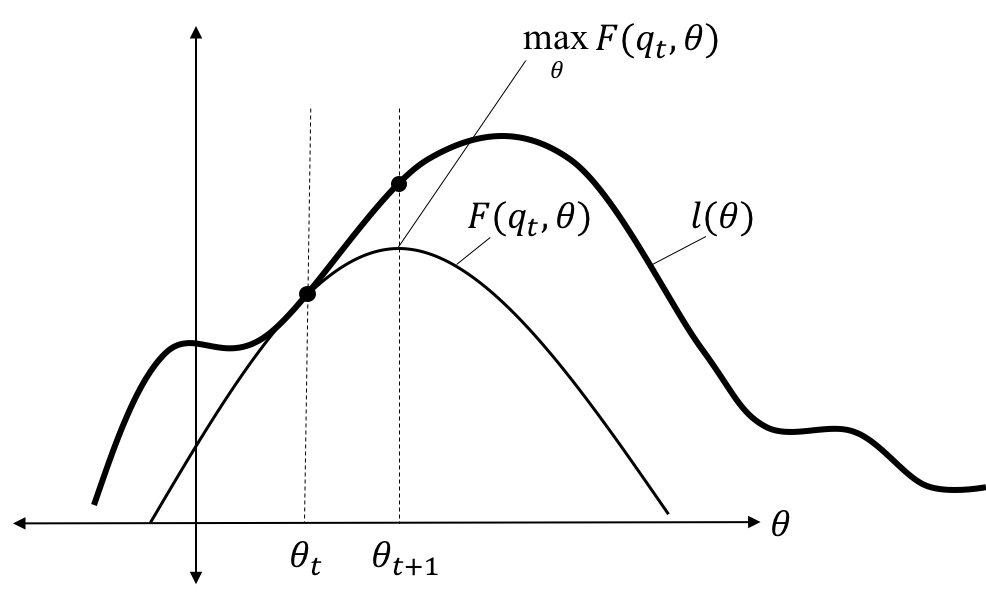
\includegraphics[scale=0.7]{./Slike/em_algoritam.png}
  \caption{Prikaz rada algoritma EM.\ $l(\bm{\theta})$ odgovara nepotpunoj log-izglednosti $\log p(X | \bm{\theta})$.\ E korak algoritma maksimizira donju varijacijsku granicu $F(q(Z), \bm{\theta}^{(t)})$ s obzirom na distribuciju $q(Z)$, a M korak algoritma maksimizira istu s obzirom na parametre $\bm{\theta}$.\ Preuzeto iz \cite{bernsteinEMblog}.}
  \label{fig:em_alg}
\end{figure}

E korak algoritma maksimizacije očekivanja sada maksimizira donju varijacijsku granicu $F(q(Z), \bm{\theta}^{(t)})$ s obzirom na distribuciju $q(Z)$ uz fiksirane vrijednosti parametara $\bm{\theta}^{(t)}$.\ 
Budući da lijeva strana jednadžbe~\ref{eq:em_general_form} ne ovisi o distribuciji $q(Z)$, vidimo da je problem maksimizacije funkcije $F(q(Z), \bm{\theta}^{(t)})$ s obzirom na distribuciju $q(Z)$ ekvivalentan problemu minimizacije izraza $KL(q(Z) || p(Z | X, \bm{\theta}^{(t)}))$.\ 
Iznos KL divergencije jednak je $0$ jedino kada vrijedi:

\begin{equation}
  q(Z) = p(Z | X, \bm{\theta}^{(t)})
  \label{eq:em_e_step_q}
\end{equation}

Ovime dobivamo rješenje E koraka, a uz dobivenu distribuciju $q^{(t + 1)}(Z)$ dodatno vrijedi da je donja varijacijska granica $F(q^{(t + 1)}(Z), \bm{\theta}^{(t)})$ jednaka nepotpunoj log-izglednosti $\log p(X | \bm{\theta}^{(t)})$.\ 
Uz uvrštavanje izraza za distribuciju $q^{(t + 1)}(Z)$, donju varijacijsku granicu možemo zapisati kao:

\begin{equation}
  \begin{aligned}
    F(p(Z | X, \bm{\theta}^{(t)}), \bm{\theta}) &= \int p(Z | X, \bm{\theta}^{(t)}) \log \frac{p(X, Z | \bm{\theta})}{p(Z | X, \bm{\theta}^{(t)})} dZ \\
                         &= \int \left[ p(Z | X, \bm{\theta}^{(t)}) \log p(X, Z | \bm{\theta}) - p(Z | X, \bm{\theta}^{(t)}) \log p(Z | X, \bm{\theta}^{(t)}) \right] dZ \\
                         &= \mathbb{E}_{Z \sim p(\cdot | X, \bm{\theta}^{(t)})} \left[ \log p(X, Z | \bm{\theta}) \right] - \mathbb{E}_{Z \sim p(\cdot | X, \bm{\theta}^{(t)})} \left[\log p(Z | X, \bm{\theta}^{(t)}) \right] \\
                         &= Q(\bm{\theta} | \bm{\theta}^{(t)}) + H(p(Z | X, \bm{\theta}^{(t)}))
  \end{aligned}
  \label{eq:em_equality_of_e_step}
\end{equation}

Pri čemu $H(p(Z | X, \bm{\theta}^{(t)}))$ označava entropiju~\cite{renyi1961measures} distribucije $p(Z | X, \bm{\theta}^{(t)})$.\ Uočimo da je dobiveni izraz za donju varijacijsku granicu jednak izrazu $Q(\bm{\theta} | \bm{\theta}^{(t)})$ koji računamo u E koraku osnovne formulacije, ali uvećan za iznos entropije $H(p(Z | X, \bm{\theta}^{(t)}))$.\ 
Kada smo odredili distribuciju $q^{(t + 1)}(Z)$ koja maksimizira donju varijacijsku granicu, možemo prijeći na M korak.\ 

M korak algoritma maksimizacije očekivanja sada maksimizira donju varijacijsku granicu $F(q^{(t + 1)}(Z), \bm{\theta})$ s obzirom na parametre $\bm{\theta}$ uz fiksiranu distribuciju $q^{(t + 1)}(Z)$ dobivenu u E koraku.\
Dakle, cilj je pronaći parametre $\bm{\theta}^{(t + 1)}$ koji maksimiziraju izraz:

\begin{equation}
  \begin{aligned}
    F(p(Z | X, \bm{\theta}^{(t)}), \bm{\theta}) &= Q(\bm{\theta} | \bm{\theta}^{(t)}) + H(p(Z | X, \bm{\theta}^{(t)})) \\ 
                                                &= Q(\bm{\theta} | \bm{\theta}^{(t)}) + const. \\
  \end{aligned}
  \label{eq:em_m_step_general}
\end{equation}

Pritom je član $H(p(Z | X, \bm{\theta}^{(t)}))$ konstantan s obzirom na trenutne parametre $\bm{\theta}$, tako da on ne utječe na tijek optimizacije.\
Vidimo da je M korak općenite formulacije identičan M koraku osnovne formulacije - jedina razlika je prisutnost konstantnog člana u izrazu koji maksimiziramo.\ 
Kao i kod osnovne formulacije algoritma maksimizacije očekivanja, dobivene parametre $\bm{\theta}^{(t + 1)}$ dalje možemo iskoristiti za provođenje E koraka sljedeće iteracije.\ 

% Kod algoritma koordinatnog uspona u dvije dimenzije, u svakoj iteraciji prvo fiksiramo jednu dimenziju i optimiramo drugu, a potom fiksiramo drugu dimenziju te optimiramo prvu.\ 
% Vidimo da algoritam EM slijedi istu ideju: u E koraku fiksiramo parametre $\bm{\theta}^{(t)}$ i optimiramo distribuciju $q(Z)$, a u M koraku fiksiramo distribuciju $q(Z)^{(t + 1)}$ te optimiramo parametre $\bm{\theta}^{(t + 1)}$.\ 

Pokažimo još da provođenjem algoritma maksimizacije očekivanja postižemo monotoni rast nepotpune log-izglednosti $\log p(X | \bm{\theta})$.\ 
Na kraju E koraka raspolažemo distribucijom $q^{(t + 1)}(Z)$ uz koju vrijedi:

\begin{equation}
  \log p(X | \bm{\theta}^{(t)}) = F(q^{(t + 1)}(Z), \bm{\theta}^{(t)})
  \label{eq:em_proof_pt1}
\end{equation}

Provođenjem M koraka dobivamo parametre $\bm{\theta}^{(t + 1)}$ uz koje vrijedi:

\begin{equation}
  F(q^{(t + 1)}(Z), \bm{\theta}^{(t)}) \leq F(q^{(t + 1)}(Z), \bm{\theta}^{(t + 1)})
  \label{eq:em_proof_pt2}
\end{equation}

Gledajući da je funkcija $F(q(Z), \bm{\theta})$ donja granica log-izglednosti $\log p(X | \bm{\theta})$, vrijedi i:

\begin{equation}
  F(q^{(t + 1)}(Z), \bm{\theta}^{(t + 1)}) \leq \log p(X | \bm{\theta}^{t + 1})
  \label{eq:em_proof_pt3}
\end{equation}

Konačno, dobivamo početnu tvrdnju:

\begin{equation}
  \log p(X | \bm{\theta}^{(t)}) \leq \log p(X | \bm{\theta}^{t + 1})
  \label{eq:em_proof_final}
\end{equation}

%-------------------------------------------------------------------------------
\chapter{Transportni problem}
\label{pog:transport}


%-------------------------------------------------------------------------------
\chapter{VIBE}
\label{pog:vibe}


%-------------------------------------------------------------------------------
\chapter{Skup podataka}
\label{pog:skup}


%-------------------------------------------------------------------------------
\chapter{Eksperimenti}
\label{pog:eksperimenti}


%--- ZAKLJUČAK / CONCLUSION ----------------------------------------------------
\chapter{Zaključak}
\label{pog:zakljucak}


%--- LITERATURA / REFERENCES ---------------------------------------------------

% Literatura se automatski generira iz zadane .bib datoteke / References are automatically generated from the supplied .bib file
% Upiši ime BibTeX datoteke bez .bib nastavka / Enter the name of the BibTeX file without .bib extension
\bibliography{literatura}


%--- SAŽETAK / ABSTRACT --------------------------------------------------------

% Sažetak na hrvatskom
\begin{sazetak}
  Sažetak...
\end{sazetak}

\begin{kljucnerijeci}
  prva ključna riječ; druga ključna riječ; treća ključna riječ
\end{kljucnerijeci}


\end{document}
